\chapter{PDZ}
\label{chap:PDZ}

Nous cherchons maintenant à évaluer les performances de notre modèle CPD sur un ensemble de protéines de la famille PDZ.Nous utilisons les résultats précédents, en particulier ceux de la section ??, pour définir les valeurs des paramètres de l'optimisation du Monte-Carlo. Mais ici, nous reprenons l'optimisation des énergies de références.

 
\section{Notre ensemble de protéine PDZ} 
\label{sec:ensemble_PDZ}


    \begin{table}[!htbp]
      \centering

      \begin{tabular}{ccc}

        \toprule
        Code PDB & résidus & nombre de positions actives\\
        \cmidrule{1-3}
        1G9O  & 	9-99	 & 	76	 \\
        1IHJ  & 	13-105	 & 	82	 \\
        1N7E  & 	668-761	 & 	79	 \\
        1R6J  & 	193-273	 & 	72	 \\
        2BYG  & 	186-282	 & 	82	 \\
        3K82  & 	305-402	 & 	80	 \\
        Cask  & 	487-568	 & 	74	 \\
        Tiam1 & 	838-930	 & 	84	 \\
        \bottomrule

      \end{tabular}      
      \caption{Les protéines PDZ}
\label{tab:protéines_PDZ}      
    \end{table}


\subsection{Description}

\subsection{Requêtes Blast croisées}

\subsection{L'alignement choisi}

\subsection{Le coeur PDZ sélectionné}


\section{L'optimisation des énergies de références} 
\label{sec:optERef}
\subsection{La méthode}
Dans notre système CPD, l'état replié joue un role important parce que les séquences d'intérts sont celles obtenues en maimimsant la differentes d'energie entre d'états deplié et l'état replié .Donc c'est tres important!.
Mais l'état déplié, lui est représenté comme une chaine popypeptidique largement etendue, de telle façon que nous considerons que chaque résidue X interagie uniquement avec le backbone environnent et avec le solvant.Puis, ce modèle est ajuster empiriquement en comparant les populations de chaque type de résidues dans les séquences calculées avec les populations dans les séquences expérimentales.L'optimisation des énergies de références consiste alors à corriger ces énergies de telles facons que la populations pour un type aa donné dans les séquences calculés cohencide avec la population experimentale de ce type . IL s'agit alors d'un problème de convergence pour la suite d'itérer de proteus + ajustement.

\subsection{Seconde méthode d'itération}

\section{Résultats} 


\paragraph{Alignements Blast croisés}


    \begin{table}[!htbp]
      \centering

      \begin{tabular}{ccccccccc}

        \toprule
        Protein & 1G9O & 1IHJ & 1N7E & 1R6J & 2BYG & 3K82 & CASK & TIAM1 \\
        \cmidrule{1-9}

        1G9O &  2e-66 & 5e-10 &  0.002 & 3e-07 & 2e-11 & 1e-12 & 5e-05 & 9e-07 \\     
        1IHJ &  5e-10 & 3e-68 &  2e-07 & no &   2e-08 & 9e-14 & 4e-06 & no    \\
        1N7E &  0.002 & 2e-07 &  3e-67 & no &    3e-14 & 2e-10 & 9e-12 & 5e-05 \\
        1R6J &  3e-07 & no  &    no  &  1e-59 &  no &   1e-06 & 0.007 & no    \\
        2BYG &  2e-11 & 2e-08 &  3e-14 & no &    7e-71 & 3e-15 & 2e-07 & 5e-05 \\
        3K82 &  1e-12 & 9e-14 &  2e-10 & 1e-06 & 3e-15 & 4e-70 & 1e-07 & 6e-04 \\
        CASK &  5e-05 & 4e-06 &  9e-12 & 0.007 & 2e-07 & 1e-07 & 7e-61 & 5e-04 \\
        TIAM1 & 9e-07 &  no &    5e-05 & no  &   5e-05 & 6e-04 & 5e-04 & 1e-68 \\
        \bottomrule


      \end{tabular}      
      \caption{E-value des alignements Blast native vs native pour nos séquences PDZ. (no= pas de touche avec une E-value inférieure à 10)}
\label{tab:Xblast}      
    \end{table}


requête sur le site d'uniprot

Target database uniprot (swissprot + trEMBL)

Matrix BLOSUM62

Filtering NO

Gapped YES


Puis selection à la main -->
enveler les redondances flagrantes
 + avoir un compromis entre diversité et qualité de l'alignement
 + rester dans la zone de ce qui a déjà été fait.



    \begin{table}[!htbp]
      \centering

      \begin{tabular}{cccc}

        \toprule
        protéines & seq NB & E value seuil & \% identité \\
        \cmidrule{1-4}
     1G9O  & 63  &    10-32  &  95-67 \\
     1IHJ  & 56  &    10-10  &  95-38 \\
     1N7E  & 93  &    10-45  &  95-84 \\
     1R6J  & 86  &    10-43  &  95-85 \\
     2BYG  & 82  &    10-41  &  95-78 \\
     3K82  & 88  &    10-46  &  95-81 \\


        \bottomrule


      \end{tabular}      
      \caption{Sélection des homologues.}
\label{tab:freq_AA_ALL}      
    \end{table}


    \clearpage

   \begin{figure}[t]
     \centering
     \begin{tabular}{c}
       \includegraphics[width=17cm]{align/1G9O.png} \\
     \end{tabular}
     \caption{L'alignement 1G9O }
\label{graph:convEref}
   \end{figure}

    \clearpage

   \begin{figure}[t]
     \centering
     \begin{tabular}{c}
       \includegraphics[width=17cm]{align/1IHJ.png} \\
     \end{tabular}
     \caption{L'alignement 1IHJ }
\label{graph:convEref}
   \end{figure}

    \clearpage

   \begin{figure}[t]
     \centering
     \begin{tabular}{c}
       \includegraphics[width=17cm]{align/1N7E.png} \\
     \end{tabular}
     \caption{L'alignement 1N7E }
\label{graph:convEref}
   \end{figure}

    \clearpage

   \begin{figure}[t]
     \centering
     \begin{tabular}{c}
       \includegraphics[width=17cm]{align/1R6J.png} \\
     \end{tabular}
     \caption{L'alignement 1R6J }
\label{graph:convEref}
   \end{figure}

    \clearpage

   \begin{figure}[t]
     \centering
     \begin{tabular}{c}
       \includegraphics[width=17cm]{align/2BYG.png} \\
     \end{tabular}
     \caption{L'alignement 2BYG }
\label{graph:convEref}
   \end{figure}

    \clearpage

   \begin{figure}[t]
     \centering
     \begin{tabular}{c}
       \includegraphics[width=17cm]{align/3K82.png} \\
     \end{tabular}
     \caption{L'alignement 3K82 }
\label{graph:convEref}
   \end{figure}

    \clearpage




\paragraph{Fréquences des acides aminés}


    \begin{table}[!htbp]
      \centering

      \begin{tabular}{ccc}

        \toprule
        Groupe & acides aminés & propriétés\\
        \cmidrule{1-3}

        1   & Ala,Cys,Thr & petit\\
        2   & Ser &\\
        \cmidrule{1-3}
        3   & Glu,Asp & chargé négativement\\
        \cmidrule{1-3}
        4   & Gln,Asn & polaire\\
        \cmidrule{1-3}
        5   & Ile,Leu,Val & apolaire\\
        \cmidrule{1-3}
        6   & Met & non polaire\\
        \cmidrule{1-3}
        7   & Hip,Hid,Hie & chargé positivement\\
        8   & Arg \\
        9   & Lys \\
        \cmidrule{1-3}
        10  & Phe,Trp & aromatique\\
        11  & Tyr \\
        \cmidrule{1-3}
        12  & Gly,Pro & non mutable\\
        \bottomrule


      \end{tabular}      
      \caption{Les groupes d'acides aminés utilisés pour l'optimisation des énergies de références.}
\label{tab:AA_groupes}      
    \end{table}



    \begin{table}[!htbp]
      \centering

      \begin{tabular}{cc}

        \toprule
        acides aminés & fréquence \\
        \cmidrule{1-2}

        Ala &   0.090 \\      
        Cys &   0.028 \\  
        Thr &   0.060 \\  
        Ser &   0.071 \\  
        Glu &   0.062 \\  
        Asp &   0.044 \\  
        Gln &   0.039 \\  
        Asn &   0.055 \\  
        Ile &   0.046 \\  
        Leu &   0.075 \\  
        Val &   0.069 \\  
        Met &   0.017 \\  
        His &   0.021 \\  
        Arg &   0.047 \\  
        Lys &   0.070 \\  
        Phe &   0.035 \\  
        Trp &   0.011 \\  
        Tyr &   0.035 \\  
        Gly &   0.075 \\  
        Pro &   0.046 \\      
        \bottomrule


      \end{tabular}      
      \caption{Fréquences des acides aminés d'après dans les  protéines.}
\label{tab:AA_groupes}      
    \end{table}


    \begin{table}[!htbp]
      \centering

      \begin{tabular}{c|cc|cc}

        \toprule
        acides aminés & résidus enfouis & groupe & résidus exposés & groupe\\
        \cmidrule{1-5}

        Ala &         0.068 &       &   0.048   \\
        Cys &         0.016 &  0.147  &   0.004 & 0.135  \\    
        Thr &         0.062 &        &   0.081   \\
        \cmidrule{1-5}
        Ser &        \multicolumn{2}{c|}{0.067}     &   \multicolumn{2}{c}{0.066}  \\
        \cmidrule{1-5}
        Glu &         0.053 & 0.089        &   0.078 & 0.134 \\
        Asp &         0.035 &    &   0.055   \\
        \cmidrule{1-5}
        Gln &         0.022 & 0.051 &   0.052 & 0.117\\
        Asn &         0.028 &         &   0.064   \\
        \cmidrule{1-5}
        Ile &         0.136 & 0.362        &   0.071  \\
        Leu &         0.120 &   &   0.055 & 0.192 \\
        Val &         0.105 &         &   0.065  \\
        \cmidrule{1-5}
        Met &    \multicolumn{2}{c|}{0.027}      &  \multicolumn{2}{c}{0.018} \\
        \cmidrule{1-5}
        Hip &         0.022 &      &   0.041 \\
        Hid &         0     &  0.022 &   0    & 0.041\\
        Hie &         0     &        &   0     \\
        \cmidrule{1-5}
        Arg &        \multicolumn{2}{c|}{0.037}      &  \multicolumn{2}{c}{0.059}\\
        \cmidrule{1-5}
        Lys &        \multicolumn{2}{c|}{0.058}         &  \multicolumn{2}{c}{0.079} \\
        \cmidrule{1-5}
        Phe &         0.037 &  0.037  &   0.017 & 0.017 \\
        Trp &         0.0   &        &   0.0  \\
        \cmidrule{1-5}
        Tyr &       \multicolumn{2}{c|}{0.008}      &  \multicolumn{2}{c}{0.015}\\
        \cmidrule{1-5}
        Gly &         0.070  & 0.089 &   0.088 & 0.123\\
        Pro &         0.019  &        &   0.035  \\
        \bottomrule


      \end{tabular}      
      \caption{Les groupes d'acides aminés utilisés pour l'optimisation des énergies de références.}
\label{tab:AA_groupes}      
    \end{table}




    \begin{table}[!htbp]
      \centering

      \begin{tabular}{ccccccccc}

        \toprule
        aa & 3K82 & 2BYG & 1R6J & 1N7E & 1IHJ & 1G9O & cask & tiam1 \\
        \cmidrule{1-9}
     ALA  & 0.045  &     0.077   &    0.085   &    0.071   &    0.100   &    0.067   &    0.046  &     0.071  \\
     CYS  & 0.021  &     0.012   &    0.027   &    0.000   &    0.011   &    0.018   &    0.030  &     0.000  \\
     THR  & 0.119  &     0.056   &    0.089   &    0.070   &    0.020   &    0.032   &    0.044  &     0.030  \\
        \cmidrule{1-9}
     SER  & 0.083  &     0.073   &    0.077   &    0.079   &    0.082   &    0.046   &    0.044  &     0.048  \\
        \cmidrule{1-9}
     GLU  & 0.039  &     0.048   &    0.001   &    0.078   &    0.010   &    0.129   &    0.063  &     0.059  \\
     ASP  & 0.047  &     0.076   &    0.000   &    0.026   &    0.028   &    0.024   &    0.039  &     0.030  \\
        \cmidrule{1-9}
     ASN  & 0.062  &     0.054   &    0.048   &    0.001   &    0.004   &    0.017   &    0.007  &     0.029  \\
     GLN  & 0.021  &     0.050   &    0.000   &    0.032   &    0.027   &    0.023   &    0.014  &     0.001  \\
        \cmidrule{1-9}
     ILE  & 0.120  &     0.102   &    0.219   &    0.084   &    0.193   &    0.030   &    0.197  &     0.116  \\
     VAL  & 0.073  &     0.108   &    0.110   &    0.041   &    0.149   &    0.119   &    0.138  &     0.131  \\
     LEU  & 0.063  &     0.099   &    0.087   &    0.131   &    0.118   &    0.114   &    0.151  &     0.255  \\
        \cmidrule{1-9}
     MET  & 0.020  &     0.000   &    0.027   &    0.020   &    0.010   &    0.008   &    0.084  &     0.015  \\
        \cmidrule{1-9}
     HID  & 0.000  &     0.000   &    0.000   &    0.000   &    0.000   &    0.000   &    0.000  &     0.000  \\
     HIE  & 0.000  &     0.000   &    0.000   &    0.000   &    0.000   &    0.000   &    0.000  &     0.000  \\
     HIP  & 0.025  &     0.025   &    0.032   &    0.026   &    0.004   &    0.043   &    0.012  &     0.001  \\
        \cmidrule{1-9}
     ARG  & 0.063  &     0.012   &    0.000   &    0.047   &    0.060   &    0.106   &    0.006  &     0.029  \\
        \cmidrule{1-9}
     LYS  & 0.042  &     0.087   &    0.055   &    0.077   &    0.015   &    0.036   &    0.071  &     0.058  \\
     TRP  & 0.000  &     0.000   &    0.000   &    0.000   &    0.000   &    0.000   &    0.000  &     0.000  \\
     PHE  & 0.063  &     0.000   &    0.055   &    0.000   &    0.061   &    0.039   &    0.039  &     0.059  \\
        \cmidrule{1-9}
     TYR  & 0.000  &     0.025   &    0.000   &    0.000   &    0.003   &    0.004   &    0.000  &     0.057  \\
     GLY  & 0.062  &     0.088   &    0.080   &    0.157   &    0.065   &    0.095   &    0.000  &     0.000  \\
     PRO  & 0.021  &     0.000   &    0.000   &    0.052   &    0.032   &    0.039   &    0.006  &     0.000  \\


        \bottomrule


      \end{tabular}      
      \caption{Compositions en acides aminés des séquences expérimentales homologues aux positions enfouies et actives.}
\label{tab:freq_AA_ALL}      
    \end{table}

    \begin{table}[!htbp]
      \centering

      \begin{tabular}{ccccccccc}

        \toprule
        aa & 3K82 & 2BYG & 1R6J & 1N7E & 1IHJ & 1G9O & cask & tiam1 \\
        \cmidrule{1-9}

   ALA  & 0.056  &  0.076  &   0.039  &   0.055  &   0.020 &   0.061  &   0.019  &   0.073 \\                                         
   CYS  & 0.000  &  0.000  &   0.000  &   0.000  &   0.011 &   0.012  &   0.000  &   0.022 \\                                           
   THR  & 0.122  &  0.058  &   0.100  &   0.104  &   0.069 &   0.028  &   0.080  &   0.073 \\                                        
        \cmidrule{1-9}
   SER  & 0.076  &  0.029  &   0.080  &   0.049  &   0.072 &   0.050  &   0.053  &   0.151 \\                                          
        \cmidrule{1-9}
   GLU  & 0.025  &  0.063  &   0.061  &   0.092  &   0.081 &   0.081  &   0.099  &   0.113 \\                                           
   ASP  & 0.074  &  0.035  &   0.093  &   0.018  &   0.082 &   0.046  &   0.041  &   0.084 \\                                           
        \cmidrule{1-9}
   ASN  & 0.045  &  0.075  &   0.078  &   0.030  &   0.096 &   0.048  &   0.088  &   0.060 \\                                         
   GLN  & 0.027  &  0.012  &   0.046  &   0.035  &   0.031 &   0.061  &   0.125  &   0.051 \\                                            
        \cmidrule{1-9}
   ILE  & 0.143  &  0.057  &   0.057  &   0.151  &   0.026 &   0.022  &   0.035  &   0.048 \\                                               
   VAL  & 0.056  &  0.104  &   0.043  &   0.053  &   0.068 &   0.088  &   0.074  &   0.037 \\                                        
   LEU  & 0.025  &  0.074  &   0.022  &   0.093  &   0.034 &   0.087  &   0.040  &   0.056 \\                                          
        \cmidrule{1-9}
   MET  & 0.049  &  0.025  &   0.021  &   0.000  &   0.015 &   0.007  &   0.028  &   0.001 \\                                          
        \cmidrule{1-9}
   HID  & 0.000  &  0.000  &   0.000  &   0.000  &   0.000 &   0.000  &   0.000  &   0.000 \\                                         
   HIE  & 0.000  &  0.000  &   0.000  &   0.000  &   0.000 &   0.000  &   0.000  &   0.000 \\                                         
   HIP  & 0.050  &  0.038  &   0.044  &   0.016  &   0.029 &   0.041  &   0.081  &   0.013 \\                                        
        \cmidrule{1-9}
   ARG  & 0.024  &  0.012  &   0.066  &   0.040  &   0.060 &   0.070  &   0.119  &   0.059 \\                                          
        \cmidrule{1-9}
   LYS  & 0.074  &  0.063  &   0.066  &   0.072  &   0.103 &   0.070  &   0.084  &   0.110 \\                                          
        \cmidrule{1-9}
   TRP  & 0.000  &  0.000  &   0.000  &   0.000  &   0.000 &   0.000  &   0.000  &   0.000 \\                                         
        \cmidrule{1-9}
   PHE  & 0.022  &  0.037  &   0.030  &   0.018  &   0.005 &   0.011  &   0.006  &   0.001 \\                                         
        \cmidrule{1-9}
   TYR  & 0.000  &  0.035  &   0.000  &   0.037  &   0.003 &   0.021  &   0.001  &   0.015 \\
        \cmidrule{1-9}
   GLY  & 0.100  &  0.149  &   0.089  &   0.093  &   0.130 &   0.130  &   0.015  &   0.019 \\                                            
   PRO  & 0.025  &  0.050  &   0.054  &   0.037  &   0.055 &   0.054  &   0.002  &   0.005 \\                                         
        \bottomrule


      \end{tabular}      
      \caption{Compositions en acides aminés des séquences expérimentales homologues aux positions exposées et actives.}
\label{tab:freq_AA_ALL}      
    \end{table}


    \clearpage


    \begin{table}[!htbp]
      \centering

      \begin{tabular}{cccc}

        \toprule
        Groupe d' acides aminés & Proteus & Proteus2 & Proteus2 (T=0175)\\
        \cmidrule{1-3}

         Ala,Cys,Thr & \\
         Ser         & \\
         Glu,Asp     & \\
         Gln,Asn     & \\
         Ile,Leu,Val & \\
         Met         & \\
         Hip,Hid,Hie & \\
         Arg         & \\
         Lys         & \\
         Phe,Trp     & \\
         Tyr         & \\
         Gly,Pro     & \\
        \bottomrule


      \end{tabular}      
      \caption{Les groupes d'acides aminés utilisés pour l'optimisation des énergies de références.}
\label{tab:RefEner_groupes}      
    \end{table}



    \clearpage


    \begin{table}[!htbp]
      \centering

      \begin{tabular}{cccc}

        \toprule
        Groupe d' acides aminés & Proteus & Proteus2 & Proteus2 (T=0175)\\
        \cmidrule{1-4}


        WF  & 0.045  &  0.049  & 0.044 \\
        IVL & 0.508  &  0.526  & 0.525 \\
        ED  & 0.069  &  0.074  & 0.078 \\
        K   & 0.032  &  0.030  & 0.041 \\
        M   & 0.019  &  0.023  & 0.025 \\
        NQ  & 0.042  &  0.032  & 0.034 \\
        S   & 0.046  &  0.034  & 0.051 \\
        R   & 0.023  &  0.030  & 0.021 \\
        PG  & 0.000  &  0.000  & 0.000 \\
        ACT & 0.165  &  0.162  & 0.146 \\
        Y   & 0.027  &  0.028  & 0.018 \\
        Hhj & 0.018  &  0.008  & 0.011 \\



        \bottomrule


      \end{tabular}      
      \caption{Les énergies de références pour les positions enfouies.}
\label{tab:RefEner_groupes}      
    \end{table}



    \begin{table}[!htbp]
      \centering

      \begin{tabular}{cccc}

        \toprule
        Groupe d' acides aminés & Proteus & Proteus2 & Proteus2 (T=0175)\\
        \cmidrule{1-4}


        WF  & 0.014  & 0.026   &  0.023 \\
        IVL & 0.141  & 0.152   &  0.193 \\
        ED  & 0.175  & 0.171   &  0.173 \\
        K   & 0.129  & 0.122   &  0.098 \\
        M   & 0.017  & 0.011   &  0.015 \\
        NQ  & 0.144  & 0.132   &  0.105 \\
        S   & 0.092  & 0.080   &  0.090 \\
        R   & 0.079  & 0.096   &  0.108 \\
        PG  & 0.000  & 0.000   &  0.000 \\
        ACT & 0.139  & 0.152   &  0.130 \\
        Y   & 0.007  & 0.010   &  0.010 \\
        Hhj & 0.056  & 0.043   &  0.050 \\


        \bottomrule


      \end{tabular}      
      \caption{Les énergies de références pour les positions exposées.}
\label{tab:RefEner_groupes}      
    \end{table}


    \clearpage


   \begin{figure}[t]
     \centering
     \begin{tabular}{cc}
       \includegraphics[width=8.45cm]{proteus/optEner_gexposed.png} &
       \includegraphics[width=8.45cm]{proteus/optEner_gburied.png} \\
     \end{tabular}
     \caption{variations des énergies de références pour les groupes de résidus, pendant de l'optimisation}
\label{graph:convEref}
   \end{figure}


   \begin{figure}[t]
     \centering
     \begin{tabular}{cc}
       \includegraphics[width=8.45cm]{new_proteus/optEner_gexposed.png} &
       \includegraphics[width=8.45cm]{new_proteus/optEner_gburied.png} \\

     \end{tabular}
     \caption{variations des énergies de références pour les groupes de résidus, pendant de l'optimisation(proteus V2)}
\label{graph:convEref2}
   \end{figure}



    \clearpage
   \paragraph{Résultats Superfamily}



    \begin{table}[h]
           \raggedleft{}

      \begin{tabular}{cccccc}

        \toprule
        Protein & Match/seq & Superfamily & Superfamily & Family & Family \\
                & size      & Evalue      & success     & Evalue & success\\
        \cmidrule{1-6}
        1G9O  & 78/91 & 3.6e-7  &  10000 & 5.0e-3  & 10000 \\
        1IHJ  & 82/94 & 4.7e-8  &  10000 & 2.4e-3  & 10000 \\
        1N7E  & 79/95 & 6.05e-6 &  10000 & 1.8e-3  & 10000 \\
        1R6J  & 61/82 & 5.6e-2  &   9775 & 9.3e-3  &  9775 \\
        2BYG  & 77/97 & 4.4e-5  &  10000 & 4.2e-3  & 10000 \\
        3K82  & 81/97 & 6.3e-11 &  10000 & 3.4e-3  & 10000 \\
        CASK  & 51/83 & 9.9e-2  &   9993 & 1.9e-2  &  9993 \\
        TIAM1 & 51/94 & 6.2e-1  &   4996 & 9.6e-3  &  4944 \\
        \bottomrule        
      \end{tabular}   
     \caption{Résultats Superfamily pour les séquences Proteus avec l'ancien test Monte Carlo}   
\label{tab:superfamily_Old_MCtest}       
\end{table}



    \begin{table}[h]
           \raggedleft{}

      \begin{tabular}{cccccc}

        \toprule
        Protein & Match/seq & Superfamily & Superfamily & Family & Family \\
                & size      & Evalue      & success     & Evalue & success\\
        \cmidrule{1-6}
        1G9O  & 77/91 & 1.3e-4  &  9999 & 3.2e-3 &  9999  \\
        1IHJ  & 81/94 & 3.9e-6  &  9999 & 2.8e-3 &  9999  \\
        1N7E  & 79/95 & 4.8e-6  & 10000 & 1.8e-3 & 100000 \\
        1R6J  & 58/82 & 2.1e-1  &  8716 & 1.3e-2 &  8716  \\
        2BYG  & 78/97 & 4.6e-3  &  9998 & 4.1e-3 &  9998  \\
        3K82  & 84/97 & 4.0e-4  &  9998 & 3.8e-3 &  9998  \\
        CASK  & 50/83 & 2.5e-1  &  7571 & 2.2e-2 &  7571  \\
        TIAM1 & 51/94 & 7.2e-1  &  3367 & 5.8e-2 &  3367  \\
        \bottomrule        
      \end{tabular}   
     \caption{Résultats Superfamily pour les séquences Proteus avec le nouveau test Monte Carlo}   
\label{tab:superfamily_Old_MCtest}       
\end{table}



    \begin{table}[h]
           \raggedleft{}

      \begin{tabular}{cccccc}

        \toprule
        Protein & Match/seq & Superfamily & Superfamily & Family & Family \\
                & size      & Evalue      & success     & Evalue & success\\
        \cmidrule{1-6}
        1G9O  & 79/91 & 3.6e-7   &  10000 & 5.0e-3 &  9999  \\
        1IHJ  & 83/94 & 4.4e-8   &  9998  & 2.4e-3 &  9998  \\
        1N7E  & 78/95 & 6.05e-6  &  9999  & 1.8e-3 & 9999   \\
        1R6J  & 61/82 & 5.6e-2   &  7721  & 9.3e-3 &  7716  \\
        2BYG  & 75/97 & 4.3e-5   &  9993  & 4.2e-3 &  9993  \\
        3K82  & 84/97 & 6.3e-11  &  9999  & 3.4e-3 &  9999  \\
        CASK  & 44/83 & 9.9e-2   &  6981  & 1.9e-2 &  6977  \\
        TIAM1 & 45/94 & 6.2e-1   &  151   & 9.2e-2 &  151  \\
        \bottomrule        
      \end{tabular}   
     \caption{Résultats Superfamily pour les séquences Proteus avec le nouveau (T=0.175) test Monte Carlo}   
\label{tab:superfamily_Old_MCtest}       
\end{table}




    \begin{table}[h]
           \raggedleft{}

      \begin{tabular}{cccccc}

        \toprule
        Protein & Match/seq & Superfamily & Superfamily & Family & Family \\
                & size      & Evalue      & success     & Evalue & success\\
        \cmidrule{1-6}
        1G9O  & 79/91 & 1.3e-9  & 10000 & 3.1e-3 &  10000  \\
        1IHJ  & 84/94 & 8.7e-8  & 10000 & 2.2e-3 &  10000  \\
        1N7E  & 77/95 & 2.1e-3  & 10000 & 2.6e-3 &  10000  \\
        1R6J  & 57/82 & 3.2e-1  & 7224  & 1.7e-2 &   7224  \\
        2BYG  & 79/97 & 6.7e-4  & 10000 & 4.2e-3 &  10000  \\
        3K82  & 84/97 & 3.7e-13 & 10000 & 2.9e-3 &  10000  \\
        CASK  & 40/83 & 1.6e-1  &  6299 & 1.8e-2 &  6299   \\
        TIAM1 & 51/94 & 1.9     &  24   & 1.2e-2 &  24     \\
        \bottomrule        
      \end{tabular}   
     \caption{Résultats Superfamily nouveau Proteus et nouvelles energies de references}   
\label{tab:superfamily_Old_MCtest}       
\end{table}







    \begin{table}[h]
           \raggedleft{}

      \begin{tabular}{cccccc}

        \toprule
        Protein & Match/seq & Superfamily & Superfamily & Family & Family \\
                & size      & Evalue      & success     & Evalue & success\\
        \cmidrule{1-6}
        1G9O  & 79/91   &    1.3e-13 & 10000 & 2.2e-3 & 10000 \\
        1IHJ  & 85/94   &    7.4e-14 & 10000 & 3.7e-3 & 10000 \\
        1N7E  & 84/95   &    2.2e-10 & 10000 & 1.2e-3 & 10000 \\
        1R6J  & 76/82   &    7.3e-13 & 10000 & 1.8e-3 & 10000 \\
        2BYG  & 86/97   &    1.3e-9  & 10000 & 9.6e-4 & 10000 \\
        3K82  & 90/97   &    3.7e-23 & 10000 & 5.2e-4 & 10000 \\
        CASK  & 68/83   &    3.5e-3  &  9925 & 7.2e-3 &  9925 \\
        TIAM1 & 65/94   &    2.3e-2  &  9775 & 2.8e-2 &  9769 \\
        \bottomrule        
      \end{tabular}   
     \caption{Résultats Superfamily pour les séquences Rosetta des  protéines PDZ}   
\label{tab:superfamily_bestRE}       
\end{table}



    \begin{table}[!htbp]
      \centering

     \caption{Alignement PDZ positions du coeur}   

      \begin{tabular}{cccccccccccccccc}

        \toprule

        \cmidrule{1-16}
   
          
1G9O & C & Y & F & L & I & A & L & L & V & V & V & I & V & L & V \\
     & 15 & 24 & 26 & 28 & 39 & 48 & 53 & 59 & 62 & 67 & 75 & 79 & 86 & 88 & 90 \\ 
1IHJ & V & F & I & I & I & A & L & I & L & V & V & I & I & L & I \\ 
     & 18 & 28 & 30 & 32 & 50 & 59 & 65 & 71 & 74 & 79 & 87 & 91 & 98 & 100 & 102 \\ 
1N7E & V & L & I & I & I & A & I & I & I & L & A & L & V & L & I \\
     & 673 & 682 & 684 & 686 & 698 & 707 & 713 & 719 & 722 & 727 & 735 & 739 & 746 & 748 & 750 \\ 
1R6J & I & V & F & F & I & A & L & I & I & V & I & L & V & I & I \\ 
     & 199 & 209 & 211 & 213 & 218 & 227 & 232 & 238 & 241 & 246 & 254 & 258 & 265 & 267 & 269 \\ 
2BYG & I & L & F & I & V & A & L & L & V & L & A & L & V & L & V \\ 
     & 194 & 203 & 205 & 207 & 224 & 233 & 239 & 245 & 248 & 253 & 261 & 265 & 272 & 274 & 276 \\ 
3K82 & I & L & F & I & I & A & L & I & V & L & A & L & V & I & A \\ 
     & 314 & 323 & 325 & 327 & 338 & 347 & 353 & 359 & 362 & 367 & 375 & 379 & 386 & 388 & 390 \\ 
CASK & F & M & I & L & V & I & L & I & I & V & L & L & I & F & I \\ 
     & 493 & 501 & 503 & 505 & 515 & 524 & 530 & 536 & 539 & 544 & 552 & 556 & 563 & 565 & 567 \\ 
Tiam1 & I & Y & F & L & V & A & L & I & I & A & L & L & L & L & V \\ 
      & 848 & 858 & 860 & 862 & 875 & 884 & 889 & 895 & 898 & 903 & 911 & 915 & 920 & 922 & 924 \\
          
   \bottomrule


   \end{tabular}     
\label{tab:corePDZ}      
    \end{table}



    \clearpage

   \begin{figure}[t]
     \centering
     \begin{tabular}{c}
       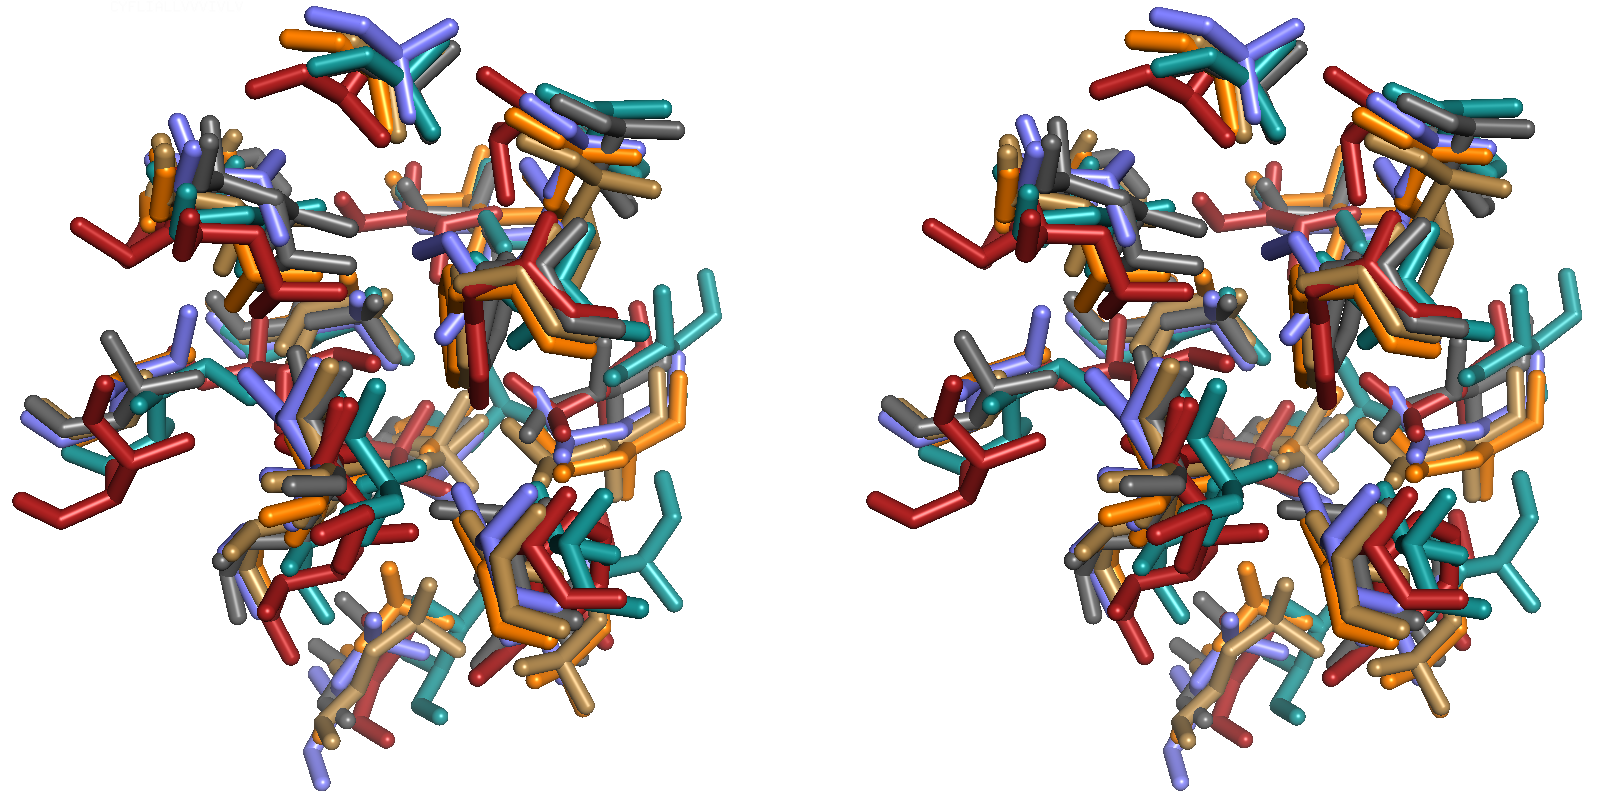
\includegraphics[width=17cm]{corePDZ.png} \\
     \end{tabular}
     \caption{le coeur PDZ sélectionné}
\label{graph:corePDZ}
   \end{figure}

    \clearpage





   \begin{figure}[t]
     \centering
     \begin{tabular}{cc}
       \includegraphics[width=8.45cm]{proteus/1G9O_core_simil.png} &
       \includegraphics[width=8.45cm]{proteus/1IHJ_core_simil.png} \\
       \includegraphics[width=8.45cm]{proteus/1N7E_core_simil.png} &
       \includegraphics[width=8.45cm]{proteus/1R6J_core_simil.png} \\

     \end{tabular}
     \caption{Similarité des séquences Proteus et Rosetta à l'alignement Pfam seed}
\label{graph:Simil_Proteus_PDZ}
   \end{figure}



   \begin{figure}[t]
     \centering
     \begin{tabular}{cc}
       \includegraphics[width=8.45cm]{proteus/2BYG_core_simil.png} &
       \includegraphics[width=8.45cm]{proteus/3K82_core_simil.png} \\ 
       \includegraphics[width=8.45cm]{proteus/CASK_core_simil.png} &
       \includegraphics[width=8.45cm]{proteus/TIAM1_core_simil.png} \\ 

     \end{tabular}
     \caption{Similarité des séquences Proteus et Rosetta à l'alignement Pfam seed (suite)}
\label{graph:Simil_Proteus_PDZ}
   \end{figure}




   \begin{figure}[t]
     \centering
     \begin{tabular}{cc}
       \includegraphics[width=8.45cm]{new_proteus/1G9O_core_simil.png} &
       \includegraphics[width=8.45cm]{new_proteus/1IHJ_core_simil.png} \\
       \includegraphics[width=8.45cm]{new_proteus/1N7E_core_simil.png} &
       \includegraphics[width=8.45cm]{new_proteus/1R6J_core_simil.png} \\

     \end{tabular}
     \caption{Similarité des séquences Proteus2 et Rosetta à l'alignement Pfam seed}
\label{graph:Simil_Proteus_PDZ}
   \end{figure}



   \begin{figure}[t]
     \centering
     \begin{tabular}{cc}
       \includegraphics[width=8.45cm]{new_proteus/2BYG_core_simil.png} &
       \includegraphics[width=8.45cm]{new_proteus/3K82_core_simil.png} \\ 
       \includegraphics[width=8.45cm]{new_proteus/CASK_core_simil.png} &
       \includegraphics[width=8.45cm]{new_proteus/TIAM1_core_simil.png} \\ 

     \end{tabular}
     \caption{Similarité des séquences Proteus2 et Rosetta à l'alignement Pfam seed (suite)}
\label{graph:Simil_Proteus_PDZ}
   \end{figure}


    \clearpage



   \begin{figure}[t]
     \centering
     \begin{tabular}{cc}
       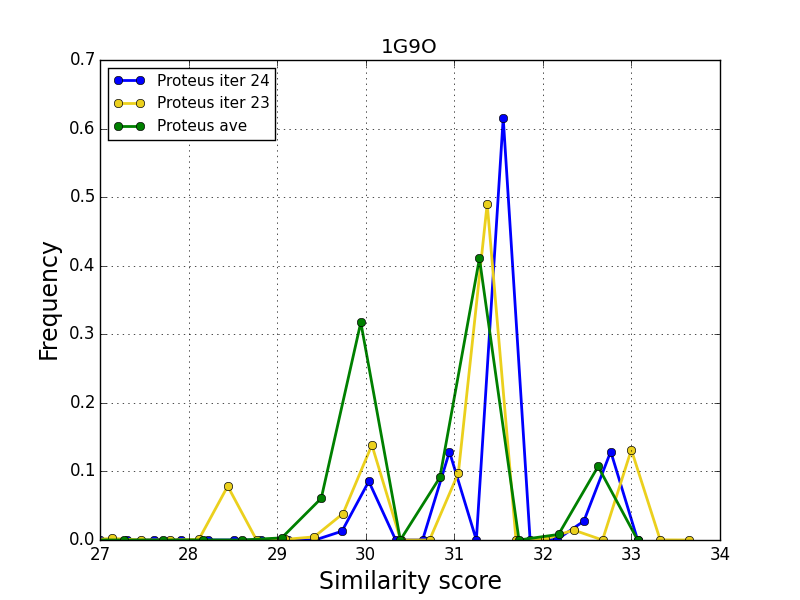
\includegraphics[width=9.45cm]{proteus/1G9O_simil_iter.png} &
       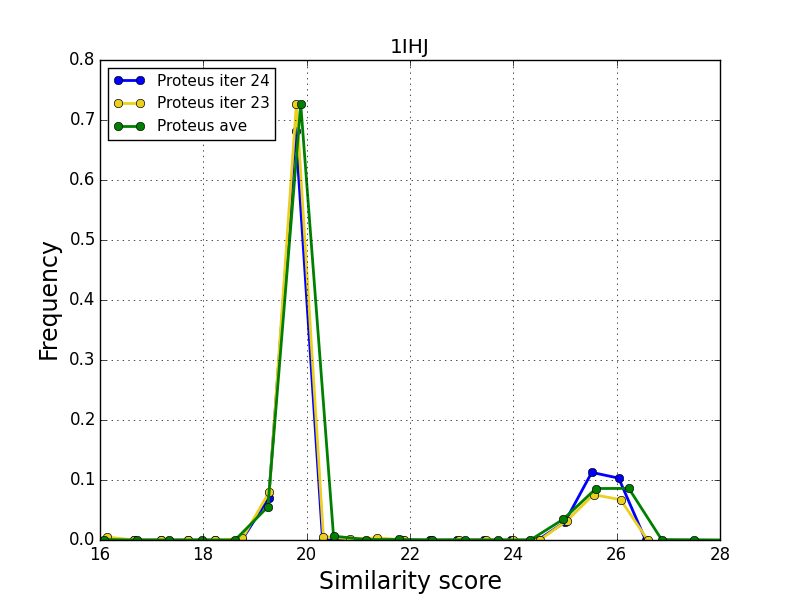
\includegraphics[width=9.45cm]{proteus/1IHJ_simil_iter.png} \\
       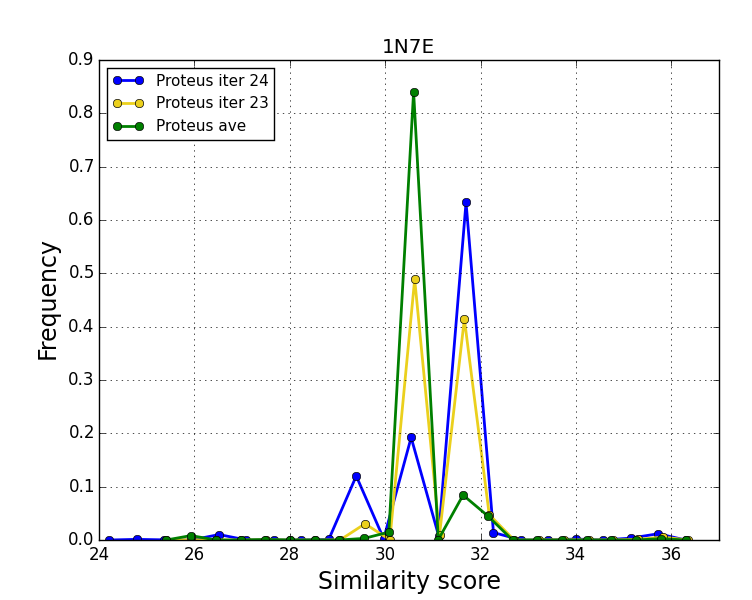
\includegraphics[width=9.45cm]{proteus/1N7E_simil_iter.png} &
       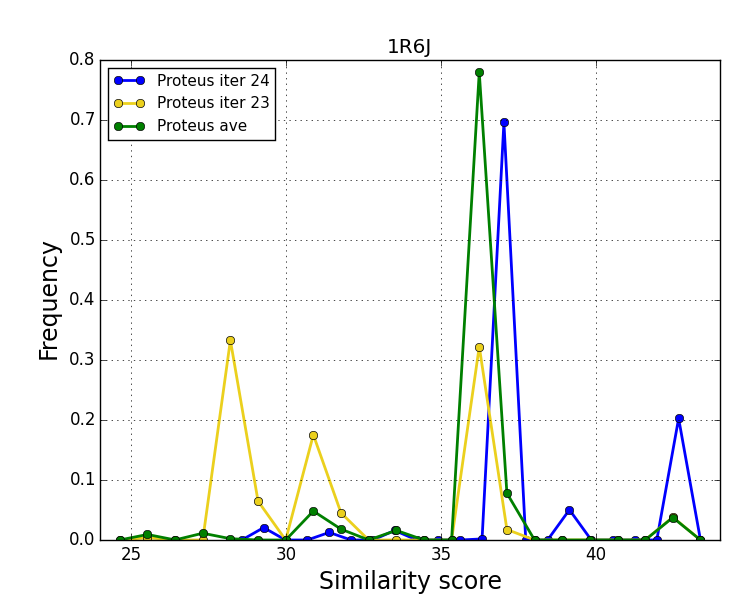
\includegraphics[width=9.45cm]{proteus/1R6J_simil_iter.png} \\

     \end{tabular}
     \caption{Similarité des séquences Proteus à l'alignement Pfam seed}
\label{graph:Simil_Proteus_PDZ}
   \end{figure}



   \begin{figure}[t]
     \centering
     \begin{tabular}{cc}
       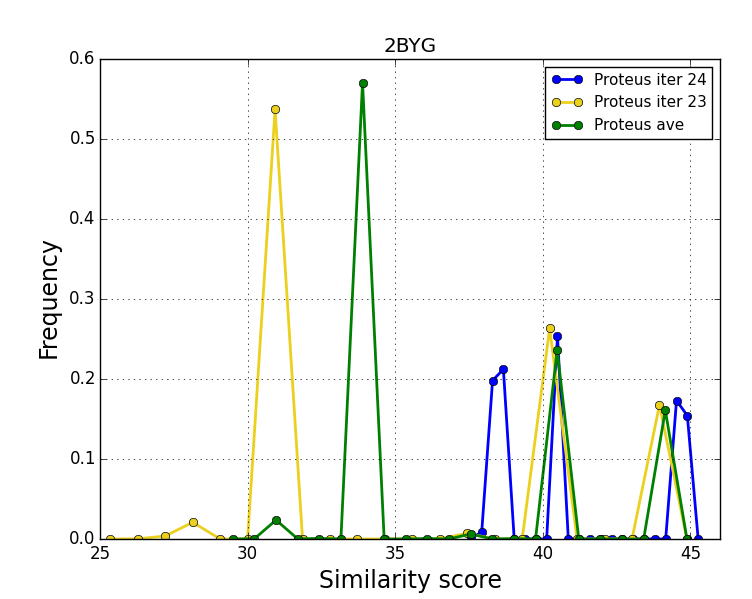
\includegraphics[width=9.45cm]{proteus/2BYG_simil_iter.png} &
       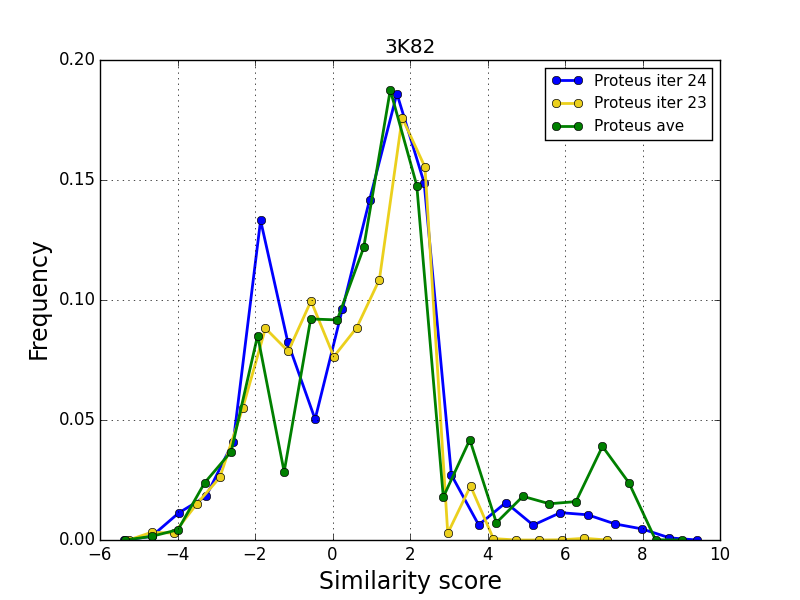
\includegraphics[width=9.45cm]{proteus/3K82_simil_iter.png} \\ 
       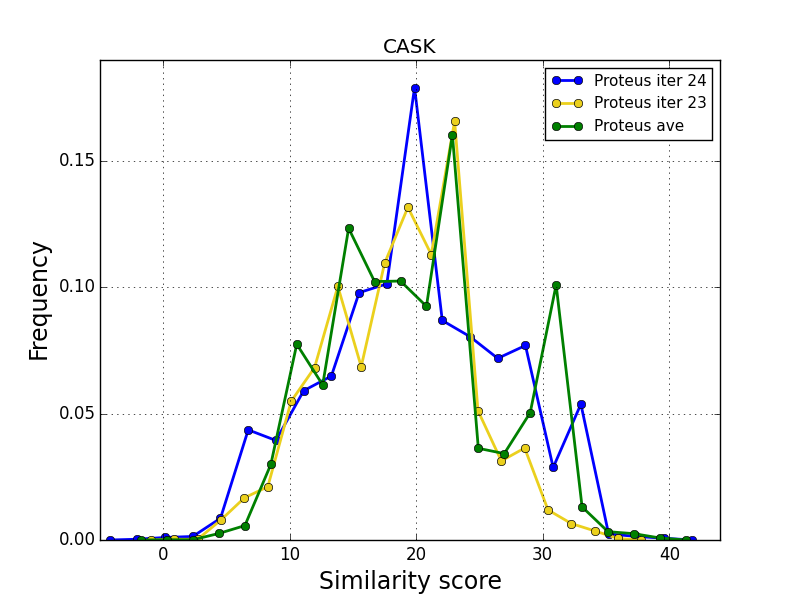
\includegraphics[width=9.45cm]{proteus/CASK_simil_iter.png} &
       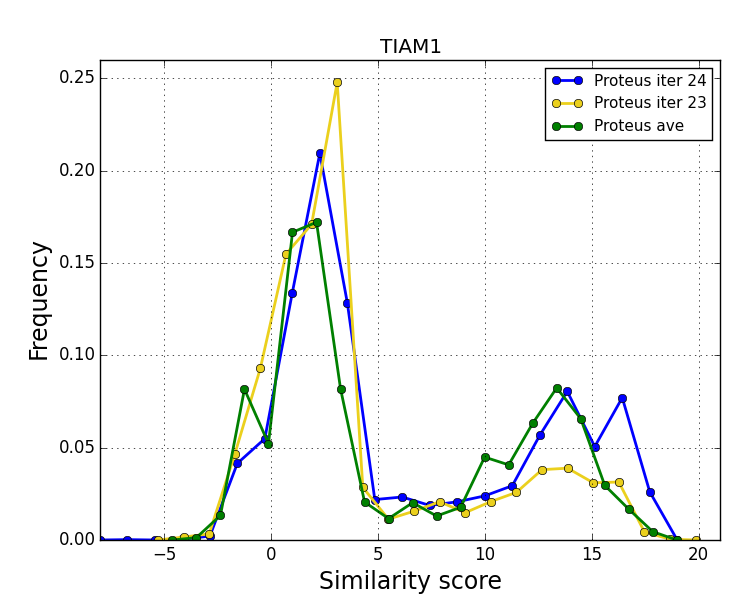
\includegraphics[width=9.45cm]{proteus/TIAM1_simil_iter.png} \\ 

     \end{tabular}
     \caption{Similarité des séquences Proteus à l'alignement Pfam seed(suite)}
\label{graph:Simil_Proteus_PDZ}
   \end{figure}


    \clearpage

    \begin{table}[!htbp]
      \centering

      \begin{tabular}{ccccccc}

        \toprule
        Protein & Proteus &  Proteus2 &  Proteus3 & Rosetta & Pfam seed \\
        \cmidrule{1-6}
        1G9O  & 1.40 & 1.42 & 1.47 & 1.45 & 3.15  \\
        1IHJ  & 1.38 & 1.46 & 1.51 & 1.55 & 3.06  \\
        1N7E  & 1.37 & 1.37 & 1.69 & 1.44 & 3.09  \\
        1R6J  & 1.39 & 1.44 & 1.53 & 1.43 & 3.03  \\
        2BYG  & 1.27 & 1.30 & 1.78 & 1.57 & 3.11  \\
        3K82  & 1.28 & 1.40 & 1.50 & 1.40 & 3.15  \\
        CASK  & 1.45 & 1.95 & 1.62 & 1.68 & 3.15  \\
        TIAM1 & 1.35 & 1.62 & 1.72 & 1.57 & 3.15  \\
        \bottomrule

      \end{tabular}      
      \caption{Moyenne de l'exponentiel de l'entropie sur les ensembles des positions des protéines}
\label{tab:Entropie_PDZ}      
    \end{table}


    \clearpage

   \begin{figure}[t]
     \centering
     \begin{tabular}{c}
       \includegraphics[width=17cm]{result/1G9O.png} \\
     \end{tabular}
     \caption{Sélection de séquences proteus 1G9O }
\label{result:1G9O}
   \end{figure}

   \begin{figure}[t]
     \centering
     \begin{tabular}{c}
       \includegraphics[width=17cm]{result/1IHJ.png} \\
     \end{tabular}
     \caption{Sélection de séquences proteus 1IHJ }
\label{result:1IHJ}
   \end{figure}

    \clearpage
   \begin{figure}[t]
     \centering
     \begin{tabular}{c}
       \includegraphics[width=17cm]{result/1N7E.png} \\
     \end{tabular}
     \caption{Sélection de séquences proteus 1N7E }
\label{result:1N7E}
   \end{figure}

   \begin{figure}[t]
     \centering
     \begin{tabular}{c}
       \includegraphics[width=17cm]{result/1R6J.png} \\
     \end{tabular}
     \caption{Sélection de séquences proteus 1R6J }
\label{result:1R6J}
   \end{figure}

    \clearpage

   \begin{figure}[t]
     \centering
     \begin{tabular}{c}
       \includegraphics[width=17cm]{result/2BYG.png} \\
     \end{tabular}
     \caption{Sélection de séquences proteus 2BYG }
\label{result:2BYG}
   \end{figure}

   \begin{figure}[t]
     \centering
     \begin{tabular}{c}
       \includegraphics[width=17cm]{result/3K82.png} \\
     \end{tabular}
     \caption{Sélection de séquences proteus 3K82 }
\label{result:3K82}
   \end{figure}

    \clearpage

   \begin{figure}[t]
     \centering
     \begin{tabular}{c}
       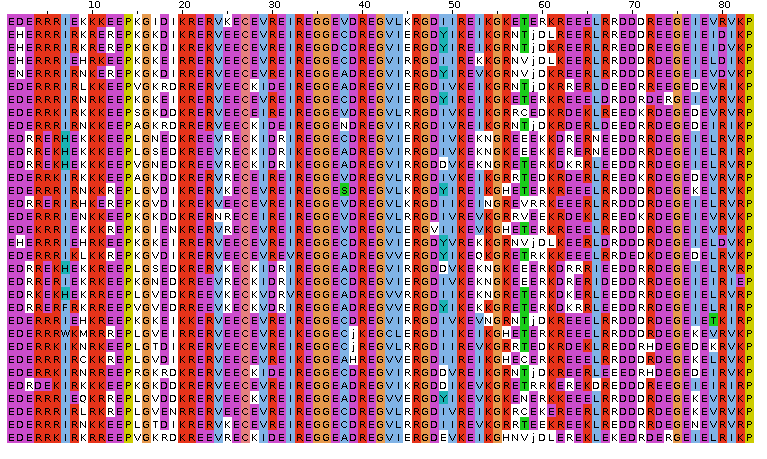
\includegraphics[width=17cm]{result/CASK.png} \\
     \end{tabular}
     \caption{Sélection de séquences proteus CASK }
\label{result:CASK}
   \end{figure}

   \begin{figure}[t]
     \centering
     \begin{tabular}{c}
       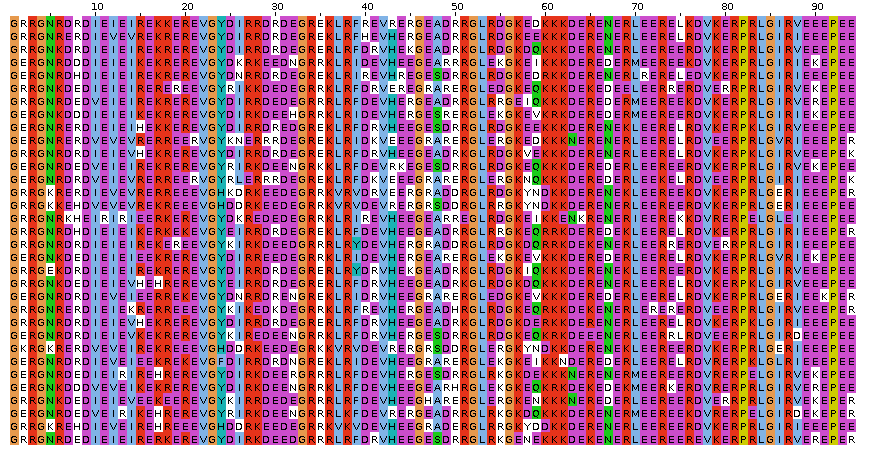
\includegraphics[width=17cm]{result/TIAM1.png} \\
     \end{tabular}
     \caption{Sélection de séquences proteus TIAM1 }
\label{result:TIAM1}
   \end{figure}

    \clearpage


   \begin{figure}[t]
     \centering
     \begin{tabular}{c}
       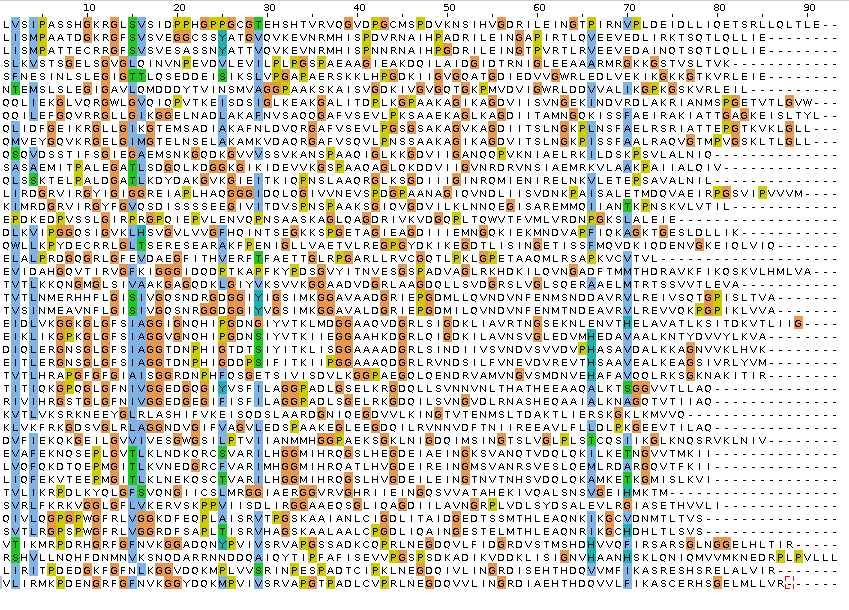
\includegraphics[width=17cm]{result/PDZ.png} \\
     \end{tabular}
     \caption{Les séquences de l'alignement PDZ seed de Pfam}
\label{result:PDZ_seed}
   \end{figure}

    \clearpage

   \begin{figure}[t]
     \centering
     \begin{tabular}{c}
       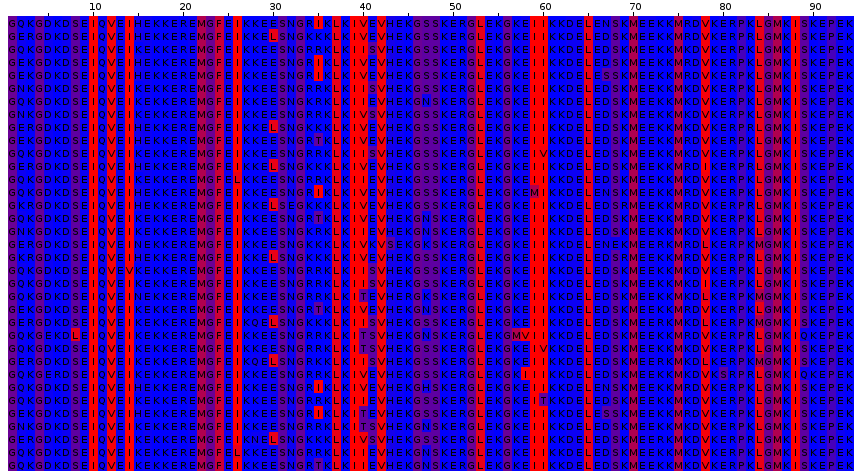
\includegraphics[width=17cm]{Tiam1/boostHydro0.png} \\
     \end{tabular}
     \caption{Séquences Tiam1 obtenues avec un delta d'énergies de références à -0,4.}
\label{result:PDZ_seed}
   \end{figure}

   \begin{figure}[t]
     \centering
     \begin{tabular}{c}
       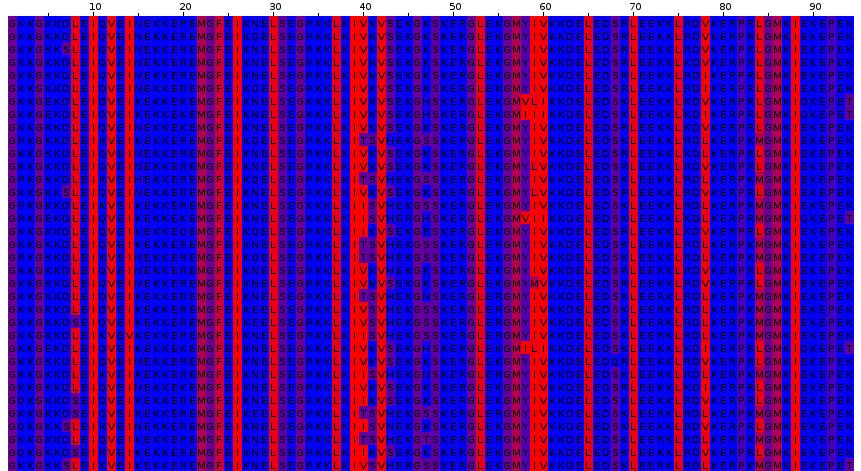
\includegraphics[width=17cm]{Tiam1/boostHydro1.png} \\
     \end{tabular}

     \caption{Séquences Tiam1 obtenues avec un delta d'énergies de références à -0,2.}
\label{result:PDZ_seed}
   \end{figure}

    \clearpage


   \begin{figure}[t]
     \centering
     \begin{tabular}{c}
       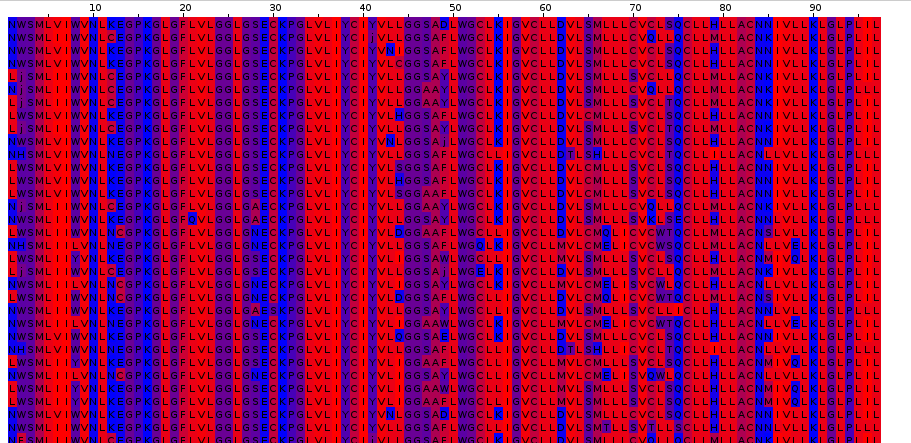
\includegraphics[width=17cm]{Tiam1/boostHydro2.png} \\
     \end{tabular}
     \caption{Séquences Tam1 obtenues avec un delta d'énergies de références à -0,1.}
\label{result:PDZ_seed}
   \end{figure}

   \begin{figure}[t]
     \centering
     \begin{tabular}{c}
       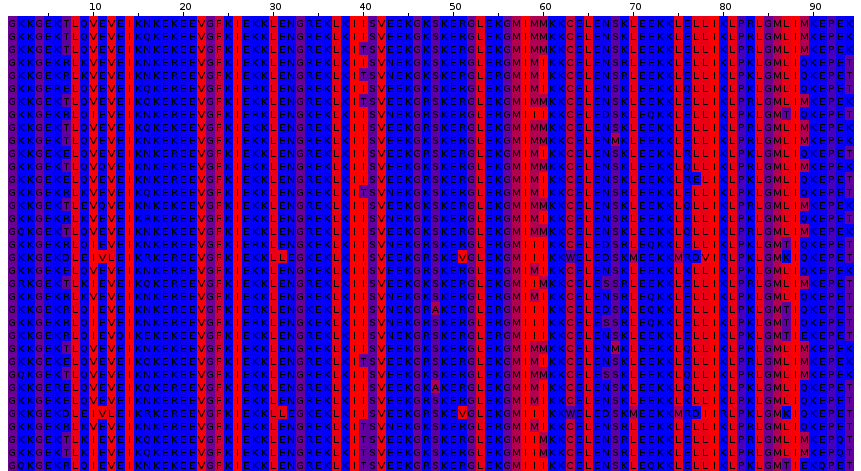
\includegraphics[width=17cm]{Tiam1/boostHydro3.png} \\
     \end{tabular}
     \caption{Séquences Tiam1 obtenues avec un delta d'énergies de références à 0.}
\label{result:PDZ_seed}
   \end{figure}

    \clearpage



   \begin{figure}[t]
     \centering
     \begin{tabular}{c}
       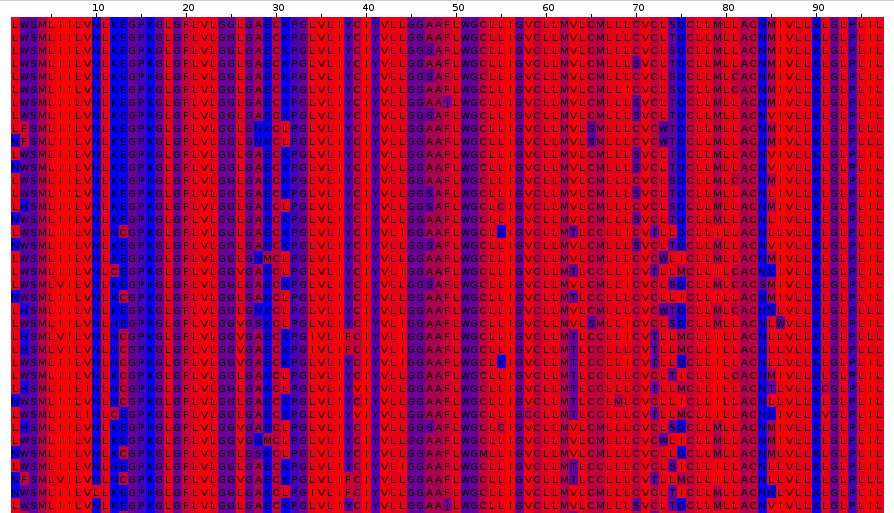
\includegraphics[width=17cm]{Tiam1/boostHydro4.png} \\
     \end{tabular}
     \caption{Séquences Tiam1 obtenues avec un delta d'énergies de références à 0,1.}
\label{result:PDZ_seed}
   \end{figure}

   \begin{figure}[t]
     \centering
     \begin{tabular}{c}
       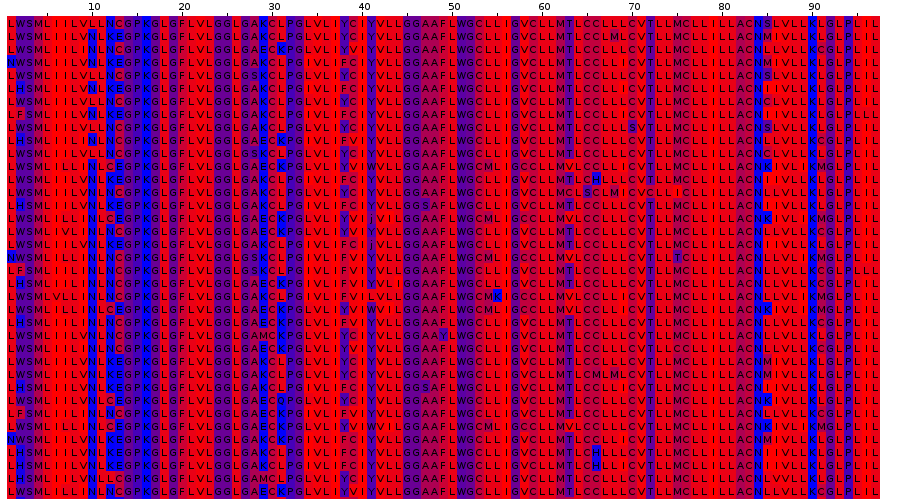
\includegraphics[width=17cm]{Tiam1/boostHydro5.png} \\
     \end{tabular}
     \caption{Séquences Tiam1 obtenues avec un delta d'énergies de références à 0,2.}
\label{result:PDZ_seed}
   \end{figure}

    \clearpage


   \begin{figure}[t]
     \centering
     \begin{tabular}{c}
       \includegraphics[width=17cm]{Tiam1/boostHydro6.png} \\
     \end{tabular}
     \caption{Séquences Tiam1 obtenues avec un delta des énergies de références  à 0,4.}
\label{result:PDZ_seed}
   \end{figure}


   \begin{figure}[t]
     \centering
     \begin{tabular}{c}
       \includegraphics[width=17cm]{2BYG/boostHydro0.png} \\
     \end{tabular}
     \caption{Séquences 2BYG obtenues avec un delta d'énergies de références à -0,4.}
\label{result:PDZ_seed}
   \end{figure}

   \begin{figure}[t]
     \centering
     \begin{tabular}{c}
       \includegraphics[width=17cm]{2BYG/boostHydro1.png} \\
     \end{tabular}
     \caption{Séquences 2BYG obtenues avec un delta d'énergies de références à -0,2.}
\label{result:PDZ_seed}
   \end{figure}

    \clearpage



   \begin{figure}[t]
     \centering
     \begin{tabular}{c}
       \includegraphics[width=17cm]{2BYG/boostHydro2.png} \\
     \end{tabular}
     \caption{Séquences 2BYG obtenues avec un delta d'énergies de références à -0,1.}
\label{result:PDZ_seed}
   \end{figure}

   \begin{figure}[t]
     \centering
     \begin{tabular}{c}
       \includegraphics[width=17cm]{2BYG/boostHydro3.png} \\
     \end{tabular}
     \caption{Séquences 2BYG obtenues sans delta d'énergies de références.}
\label{result:PDZ_seed}
   \end{figure}

    \clearpage



   \begin{figure}[t]
     \centering
     \begin{tabular}{c}
       \includegraphics[width=17cm]{2BYG/boostHydro4.png} \\
     \end{tabular}
     \caption{Séquences 2BYG obtenues avec un delta d'énergies de références à 0,1.}
\label{result:PDZ_seed}
   \end{figure}

   \begin{figure}[t]
     \centering
     \begin{tabular}{c}
       \includegraphics[width=17cm]{2BYG/boostHydro5.png} \\
     \end{tabular}
     \caption{Séquences 2BYG obtenues avec un delta d'énergies de références à 0,2.}
\label{result:PDZ_seed}
   \end{figure}

    \clearpage


   \begin{figure}[t]
     \centering
     \begin{tabular}{c}
       \includegraphics[width=17cm]{2BYG/boostHydro6.png} \\
     \end{tabular}
     \caption{Séquences 2BYG obtenues avec un delta d'énergies de références à 0,4.}
\label{result:PDZ_seed}
   \end{figure}





%%% Local Variables:
%%% mode: latex
%%% TeX-master: "../../rapport"
%%% End:
